% 1977 年四川卷第二题：半径 R、中心角 120° 的扇形卷成圆锥容器
% 扇形顶点在左、弧张向右下（标弧长 C、圆心角 120°），
% 圆锥立在其上（虚线标高 h 与底面半径 r，母线即扇形半径 R）（按源卷第 3 页布局）
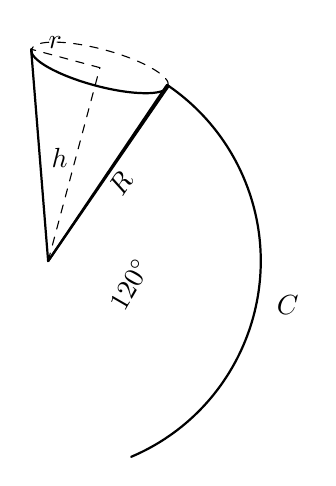
\begin{tikzpicture}[scale=0.9,line cap=round]
  % 圆锥（锥顶与扇形顶点重合）
  \coordinate (V) at (0,0);
  \coordinate (M) at (0.73,2.73);   % 底面椭圆中心（h=2.83，沿 75° 轴）
  \coordinate (P1) at (-0.24,2.99); % 底面椭圆左端
  \coordinate (P2) at (1.70,2.47);  % 底面椭圆右端（与扇形上半径共线）
  \draw[thick] (V)--(P1);
  \draw[thick] (V)--(P2);
  \begin{scope}[shift={(0.73,2.73)},rotate=-15]
    \draw[dashed] (1,0) arc (0:180:1 and 0.26);   % 底面椭圆后半（虚线）
    \draw[thick] (-1,0) arc (180:360:1 and 0.26); % 底面椭圆前半（实线）
\end{scope}
  % 高 h 与底面半径 r（虚线）
  \draw[dashed] (V)--(M);
  \node at (0.16,1.45) {$h$};
  \draw[dashed] (M)--(P1);
  \node at (0.10,3.08) {$r$};
  % 扇形（上半径与圆锥母线 V-P2 重合，标 R；下半径向右下，标弧长记号 C）
  \draw[thick] (V)--(56:3);
  \draw[thick] (-67:3) arc[start angle=-67, end angle=56, radius=3];
  \node[rotate=56] at (1.02,1.10) {$R$};
  \node[rotate=60] at (1.15,-0.32) {$120^\circ$};
  \node at (3.38,-0.62) {$C$};
\end{tikzpicture}
